\documentclass[a4paper, punct,space,nospace, fancyhdr, fntef,UTF8]{ctexart}

% \usepackage{ctex} % 使用中文包

\usepackage{DGUT} % 使用东莞理工论文样式


%%%%%%%%%%%% Begin Documents %%%%%%%%
\begin{document}
    % 论文中文标题
\def\thesistitlezh{基于OpenCV的工程图数据提取及其在UWB定位系统的应用}


% 论文英文标题
\def\thesistitleen{Data extraction of engineering drawings based on OpenCV and its application in the location system of UltraWideband}


% Thank Words
\def\thankwords{

此处请写致谢的内容。

它可以有多段。
}

    
    \pagestyle{empty} % 不要页脚页眉
    
% %\centerline{\kaishu\zihao{-0}{深圳大学}}
% \begin{figure}[htbp]
% 	\begin{center}
% 		\includegraphics[width=2.7in]{szu}
% 	\end{center}
% \end{figure}

\centerline{\kaishu\zihao{1}{东\ 莞\ 理\ 工\ 学\ 院}}

\vskip 1cm

\centerline{\heiti\zihao{1}{本\ 科\  毕\  业\  论\  文\  (设计)}}

\vskip 3.5cm



\begin{flushleft}
	\zihao{3}
	\hspace{3cm}{\heiti{题目:}}      
	{\kaishu\underline{\quad\textbf{基于OpenCV的工程图数据提取}\hspace{1.2cm}}}               \\
	\vspace{10bp}
	\hspace{3cm}{\kaishu\underline{\hspace{2.7cm}\quad\textbf{在UWB定位系统的应用}\hspace{2.1cm}}}
	\vspace{10bp}
	
	\hspace{3cm}{\heiti{姓名:}}      
	{\kaishu\underline{\hspace{2.8cm}\textbf{陈俊杰}\hspace{3.5cm}}}              \\
	\vspace{10bp}
	
	\hspace{3cm}{\heiti{专业:}}     
	{\kaishu\underline{\hspace{1.5cm}\textbf{软件工程}\hspace{2cm}}}            \\
	\vspace{10bp}
	
	\hspace{3cm}{\heiti{学院:}}      
	{\kaishu\underline{\hspace{1.5cm}\textbf{机器人学院}\hspace{2cm}}}               \\
	\vspace{10bp}
	
	\hspace{3cm}{\heiti{学号:}}      
	{\kaishu\underline{\hspace{2.4cm}\textbf{201541412127}\hspace{2.6cm}}}                   \\
	\vspace{10bp}
	
	\hspace{3cm}{\heiti{指导教师:}} 
	{\kaishu\underline{\hspace{1.8cm}\textbf{刘文果}\hspace{3.5cm}} }                         \\
	\vspace{10bp}
	
	\hspace{3cm}{\heiti{职称:}}      
	{\kaishu\underline{\hspace{3.2cm}\textbf{副教授}\hspace{3.8cm}} }                         \\
	
\end{flushleft}

\vskip 4cm

\centerline{\zihao{3} 2019 年 \  4 月\  20 日}
    \newpage

\centerline{\heiti\zihao{-2}{东莞理工学院本科毕业论文(设计)诚信声明}}


\vskip 3cm 


\begin{spacing}{2.0}
	\zihao{4}
本人郑重声明:所呈交的毕业论文(设计),题目《基于OpenCV的工程图数据提取及其在UWB定位系统的应用》是本人在指导教师的指导下,独立进行研究工作所取得的成果。对本文的研究做出重要贡献的个人和集体,均已在文中以明确方式注明。除此之外,本论文不包含任何其他个人或集体已经发表或撰写过的作品成果。本人完全意识到本声明的法律结果。

\vskip 3cm

{\flushright{
		毕业论文(设计)作者签名:\hspace{2.2cm}
		
		
		
		\hspace{7.5cm}{日期:\hspace{2cm}年 \hspace{.5cm}月\hspace{.5cm}日}\hspace{4cm} 
	}}
\end{spacing}



    

    \zihao{-4}
    % \tableofcontents%生成目录
    \thispagestyle{empty} %页脚不要页码
    %“目录”两个字的样式与section的样式一致,默认居中,故将设置section标题居左放置在生成目录后
    \CTEXsetup[format={\Large\bfseries}]{section}  %section标题居左
    
	%%%%正文开始,页脚有页码
	\cfoot{\zihao{-5}第 \ \thepage \ 页 \ 共 \ \pageref{lastpage} 页}%%%%lastpage为末页标签
	%正文
	\zihao{5}
	\pagenumbering{arabic}%页码使用阿拉伯数字
	\setcounter{page}{0}  %重新设置页码计数
	\pagestyle{fancy}

    % \newpage


\centerline{\fangsong\bf\zihao{-2}{基于OpenCV的工程图数据提取及其}}

\centerline{\fangsong\bf\zihao{-2}{在UWB定位系统的应用}}

\addcontentsline{toc}{section}{摘要(关键词)}%加入目录

\vskip 1cm

\begin{center}
	\kaishu
	\hspace{2cm}机器人学院软件工程专业 \quad 陈俊杰 
	\vspace{5bp}
	\newline
	学号:201541412127
\end{center}

\vskip 10bp
{
\kaishu	
\hspace{5bp}{\zihao{-4}\textbf{【摘要】}} 
本文介绍了铺砖机器人的研究背景和意义,列举了同类机器人在国内外的发展现状,肯定了铺砖机器人在未来发展的前景。本文从铺砖机器人在实际施工场地中室内定位的需求出发,提出了提取工程图数据和实时定位两个部分的解决方案。第一部分中工程图由常规的DWG格式文件转换到JPG格式图像,再经过OpenCV处理,检测出工程图中的角点,并通过角点定位排序法;第二部分利用排好序的角点,通过Qt绘制出等比例的工程图,并利用砖块对工程图进行栅格化,再将砖块信息反馈给铺砖机器人,最后利用UWB串口返回的数据通过Python和C/C++的混合编程定位机器人在室内的实时位置。


\vskip 10bp

\hspace{5bp} {\zihao{-4}\textbf{【 关键词 】}} 
铺砖机器人; DWG2JPG; PyQt5; Trilateration定位; 混合编程
}

    % \newpage

\centerline{\fangsong\bf\zihao{-2}{Data extraction of engineering drawings based}}

\centerline{\fangsong\bf\zihao{-2}{on OpenCV and its application in the}}

\centerline{\fangsong\bf\zihao{-2}{ location system of UltraWideband}}


\addcontentsline{toc}{section}{Abstract(key words)}%加入目录


\vskip 20bp

\hspace{4bp} {\zihao{-4}\textbf{【 Abstract】}} 
This paper introduces the research background and significance of Mobile Tiling Robot, and enumerate the development situation of the same kind of robot at home and abroad, sure of the prospect of Mobile Robotic Tiling in the future. This paper is starting from the demand of the indoor location for Mobile Tiling Robot in the real construction site, and put forward solutions consists of two parts : extracting data from  engineering drawings and real-time location system. The first part is convert DWG format to JPG at first, secondly process image by using OpenCV, then find out the Harris Corners, finally locate and sort the corners by algorithm. The second part is use the processed corners to plot the equal-probability engineering drawings by Qt, then rasterize the region and feedback the tile information to robot, lastly with the data returned from the serial port of UltraWideband, calculate the real-time location of Mobile Tiling Robot by using the mixed program of Python and C/C++.

\vskip 10bp

\hspace{5bp}{\zihao{-4}\textbf{【 Keywords】}}
Mobile Tiling Robot; DWG2JPG; PyQt5; Trilateration Location; Mixed Program
    % \section{引言}

\subsection{研究背景及意义}

UWB的意义

\subsection{本文主要工作}

本文从 XXX 开始说起

\subsection{论文组织结构}
 
 本论文分为 X 章,内容如下:

 第一章为引言,主要介绍了本论文的研究背景、意义,主要工作及论文的组织结构。

 第二章为

 第三章为预备工作,

 第四章为

 


	\section{相关技术及背景}

\subsection{建筑工程图的认识}
建筑工程图是用来表示房屋的规划位置、外部造型、内部布置、内外装修、细致结构、固定设施及施工要求等的图纸。它包括施工图平面图、建筑总平面图、建筑剖面图、建筑立面图和建筑详图。

工程图纸分类分为三种:建筑施工图(又称建施),主要表示房屋的总平面图、剖面图、立面图等;结构施工图(又称结施),主要表示房屋承重结构的布置、构件类型、大小、数量及做法等。它包括结构布置图和构件详图;设施施工图(又称设施),主要表示各种线路、设备和管道的布置、走向以及安装施工要求等。

而本课题采用的建筑工程图属于建筑施工图的房屋平面图(文章以下出现的“工程图”时均表示建筑平面图)。而在现今,国内建筑行业在绘制平面图普遍使用AutoCAD软件绘制成.dwg文件格式的工程图。

.dwg是AutoCAD软件保存图形及属性数据的一种二进制文件格式,是制图行业的工业标准,数据结构复杂,主要包括文件头部(HEADER)、应急头部(CON-TINGENY HEADER)、表部(TABLES)、实体部(ENTITLES)、块实体部(BLOCKS)5部分。


\subsection{OpenCV的基础知识}
\subsubsection{OpenCV介绍}
OpenCV(Open Source Computer Vision Library)诞生于Intel研究中心,其目的是开发开一个普遍可用的计算机视觉库。在Inter的性能库团队的帮助下,OpenCV实现了一些关于计算机视觉的核心代码以及算法,并在Inter俄罗斯的库团队的帮助下得到优化。

OpenCV是一个开源的是计算机计算机视觉库。OpenCV采用 C/C++语言编写,可以运行在Linux/Windows/Mac等操作系统上。OpenCV还提供了可Python、Ruby、MATLAB以及其他语言的接口。无论是科研使用还是商业使用,OpenCV都是开放源代码且免费的,OpenCV的代码可用于或者嵌入(整体或部分)其他的应用程序中。

OpenCV主体分为五个模块,其中四个模块如图1所示。还有一个模块是CvAux模块,该模块中一般存放一些新出现的实验性的算法和函数,同时还有一些即将被淘汰的算法和函数。
\begin{figure}[htbp]
    % caption放上面就会显示在图的上方,出现在下面就是出现在图的下方
    \label{gra1}
    \begin{center}
        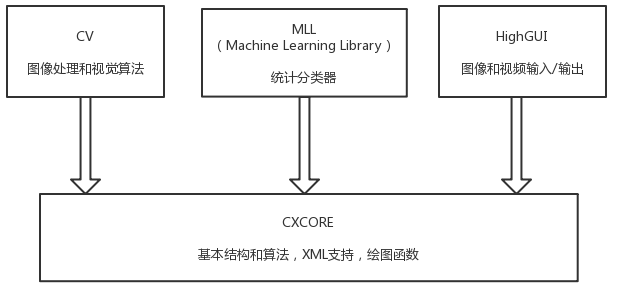
\includegraphics[width=3.6in]{OpenCV_module}
        \caption{OpenCV模块图}
    \end{center}
\end{figure}

\subsubsection{灰度处理}
% \begin{spacing}
% \subsubsubsection{灰度的概念:}
% ----------
灰度的概念:
% \end{spacing}

一个大小为$M * N$的数字图像是由$M$行$N$列的有限元素组成的,每个元素(又称为像素)都有特定的位置和幅值,代表了所在行列位置上的图像物理信息,如灰度和RBG等。

在二指图像(像素只有0和1两种取值,0代表黑色,1代表白色)中进一步加入许多介于黑色和白色之间的颜色深度,就构成了灰度图像。这类图像通常显示为从最暗黑色到最亮的白色的灰度,每种灰度(颜色深度)称为一个灰度级,通常用L表示。在灰度图像中,像素可以取0~L-1
之间的整数值,根据保存灰度数值所使用的数据类型不同,可能有256种取值或者$2^k$种取值,当k=1时即退化为二指图像。在通常情况下,图像的灰度级范围从0到255,白色为255,黑色为0,故黑白图片又称为灰度图像。灰度级越大表示越亮。

% ----------
图像灰度级分辨率:

在数字图像处理中,灰度级分辨率又称色阶,是指图像中可分辨的灰度级数目$L$,
它与存储灰度级别所使用的数据类型有关。由于灰度级度量的是投射到传感器上光辐射
值的强度,所以灰度级分辨率也叫辐射计量分辨率。

随着图像的灰度级分辨率逐渐降低,图像中包含的颜色数目变少,从而在颜色的角
度造成图像信息受损,同样使图像细节表达受到了一定的影响。

% ----------
灰度图像在图像处理中的作用:

对于一个数字图像处理系统来说,一般可以将处理流程分为3个阶段。在获取原始图像后,首先是图像预处理阶段,第二是特征抽取阶段,最后才是识别分析阶段。预处理阶段尤为重要,这个阶段处理不好则后面的工作根本无法展开。

灰度直方图是最基本的图像分析工具。灰度直方图是图像的一种统计表达,它反映了该图中不同灰度级出现的统计概率。主要应用于图像分割和图像灰度变换等处理过程中。

利用直方图辅助实现的各种灰度变换(点运算)\footnote{点运算:是指对一副图像中每个像素点的灰度值进行计算的方法。}
,包括线性灰度变换、分段线性灰度变换、非线性灰度变换等。

% ----------
阈值处理:

根据用户规定的阈值(threshold),一张图像每个像素的灰度值放在一个数组中,然后根据数值中的每个元素的值低于还是高于阈值而进行一些处理。例如阈值的二值化处理,图像中每个像素点的灰度值如果大于threshold,则这个值置为255;如果小于threshold,则将这个值置为0。

% ----------
直方图均衡化:

把原始图像的直方图变换为均匀分布的形式,从而增加图像灰度的动态范围,达到增强图像对比度的效果。经过均衡化的图像,其灰度级出现的概率相同,此时图像的熵\footnote{熵指的是体系的混乱的程度,对焦良好的图像的熵大于没有清晰对焦的图像,因此可以用熵作为一种对焦评价标准。熵越大,图像越清晰。——来源百度百科}
最大,图像所包含的信息量最大。

\begin{figure}[htbp]
    % caption放上面就会显示在图的上方,出现在下面就是出现在图的下方
    \label{gra1}
    \begin{center}
        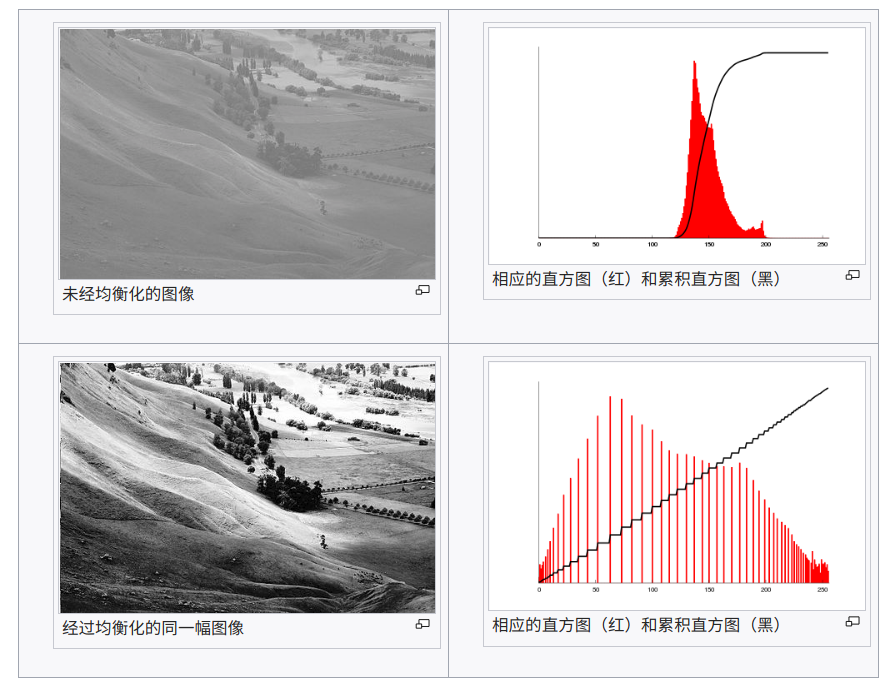
\includegraphics[width=3.6in]{Histogram_equalization}
        \caption{直方图均衡化前后对比}
    \end{center}
\end{figure}


\subsubsection{图像分割}

% -------------
图像分割概述:

图像分割是指将图像中具有特殊意义的不同区域划分出来,这些区域是互不相交的, 每个区域满足灰度、纹理、彩色等特征的某种相似性准则。

图像分割算法一般基于图像灰度值的两个基本特性之一:不连续性和相似性。第1类是基于图像灰度的不连续变化分割图像,例如图像的边缘,有边缘检测、边界跟踪、Hough变换等算法。第2类是依据事先制定的准则将图像分割为相似的区域,如阈值分割。

% ---------
图像分割的作用:

图像分割是图像识别和图像理解的前提步骤,图像分割质量的好坏直接影响了后续图像处理的效果。

\begin{figure}[htbp]
    % caption放上面就会显示在图的上方,出现在下面就是出现在图的下方
    \label{gra1}
    \begin{center}
        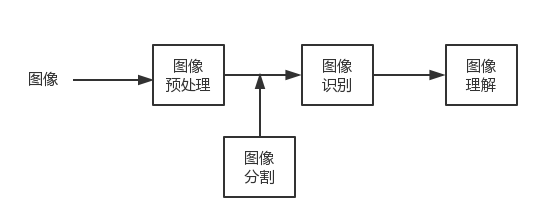
\includegraphics[width=4in]{Image_Segmentation.png}
        \caption{直方图均衡化前后对比}
    \end{center}
\end{figure}


% ----------
图像分割应用:

在交通上,应用于车辆检测、车辆跟踪、车种识别等;在生物医学上,应用于计算机断层图像CT、核磁共振、X光透视、病毒细胞的自动检测和识别等;在工业上,应用于产品的精度和纯度分析、矿藏分析、无接触式检测等;另外,在神经网络、机器人视觉、图像传输、身份鉴定等都各个领域都有着广泛的应用。


% ----------
Canny算法的步骤:

Canny边缘检测的基本思想就是首先对图像选择一定的Gauss(高斯)滤波器进行平滑滤波,然后采用非极值抑制技术进行处理得到最后的边缘图像。步骤如下:

(1)用高斯滤波器平滑图像
滤波的主要目的是降噪,高斯滤波会将图像变得模糊,同时也会可能增加边
缘的宽度。对于在图像中位置$(m,n)$的像素点,其灰度值为$f(m,n)$。

\bf{$g_{\sigma}(m,n) = \frac{1}{\sqrt{2\pi\sigma^2}} e^{\frac{-m^2+n^2}{2{\sigma^2}}} \cdot f(m,n) $}


$H_x = \begin{bmatrix} -1 & -2 & -1 \\ 0 & 0 & 0  \\ 1 & 2 & 1\end{bmatrix}$ \quad{}
$H_y = \begin{bmatrix} -1 & 0 & 1 \\ -2 & 0 & 2  \\ -1 & 0 & 1\end{bmatrix}$

$ G_x = H_y \cdot f(m,n)$ \quad{} $ G_y = H_x \cdot f(m,n)$


$G(m,n) = \sqrt{G_x(m,n) ^2 + G_y(m,n)^2}$

$\theta = arctan \frac{G_x(m,n)}{G_y(m,n)} $

\quad{}

$\rho = xcos \theta +ysin \theta$

\quad{}

$T_{TOF} =[(Ta_1 - Ta_2) - (Tb_1 - Tb_2)] /2 $ \quad{}\quad{}(1)

\quad{}

$ S= C \cdot T_{TOF}$ , \quad{}(C为光速, 即 $C=3\cdot 10^8$ ) \quad{}\quad{}(2)

\quad{}

$d_i^2 = (x - x_i)^2 + (y - y_i)^2 $ \quad{}\quad{}(1)

\quad$ = x^2 -2x_ix + x_i^2 + y^2 - 2y_iy + y_i^2$ , \quad{}其中$(i = 0,1,2)$

\quad

$d_i^2 - d_N^2 = -2x(x_i^2 - x_N^2) + x_i^2 -x_N^2 $ \quad{}\quad{}(2)

\quad\quad\quad\quad{} $- 2y(y_i-y_N) + y_i^2 - y_N^2$, \quad{}其中$(i = 0,1,2\dots, N-1)$

\quad{}

$b = \begin{bmatrix} d_1^2 - d_N^2 - (x_1^2 + y_1^2) + (x_N^2 + y_N^2) \\ d_2^2 - d_N^2 - (x_2^2 + y_2^2) + (x_N^2 + y_N^2) \\ \vdots \\d_{N-1}^2 - d_N^2 - (x_{N-1}^2 + y_{N-1}^2) + (x_N^2 + y_N^2) \\\end{bmatrix}$ \quad{}\quad{}(3)

\quad

$A = -2 \begin{bmatrix} x_1 - x_N & y_1 - y_N \\ x_2 - x_N & y_2 - y_N \\ \vdots  \\ x_{N-1} - x_N & y_{N-1} - y_N \\\end{bmatrix}$ \quad{}\quad{}(4)

\quad

$X = (A^TA)^{-1}A^Tb$ \quad{} 求解

\quad{}

$G_T(m,n) = \begin{cases}
    G(m,n), & if\quad{} G(m,n)>=T \\
    0, & $其他情况$
    
\end{cases} $

\[ y=\begin{cases}
    -x & x<0\\
    x & x\geq0
    \end{cases} \]
    

\quad

$PPI = \sqrt{1920^2 + 1080^2}/15.6 = 141.21$

\quad

$DP = 15.6 * 25.4 / \sqrt{1920^2 + 1080^2} = 0.1799$ ,(其中1英寸 = 25.4 mm)
	% \include{doc/chapter03}
	% \include{doc/chapter04}
	% \include{doc/chapter05}
	% \include{doc/chapter06}
	% \include{doc/chapter07}

\end{document}

